\documentclass[runningheads]{llncs}

%PACKAGES
\usepackage[utf8]{inputenc}
\usepackage{listings, xcolor}
\usepackage{graphicx} 
\usepackage{lipsum}
\usepackage{float}
\setcounter{secnumdepth}{5}
\begin{document}
\title{Comparing FreeST, Go and Rust}
\author{Jorge Martins\inst{1} \and
Diogo Lopes\inst{1}
}
\definecolor{darkblue}{rgb}{0.0, 0.0, 0.55}
\lstset{language=Java,
numbers=none,
keywordstyle = \color{blue},
commentstyle = \color{darkblue},
breaklines = true,
showstringspaces = false,
tabsize = 4,
basicstyle=\small,
} 
\institute{Departamento de Informática da Faculdade de Ciências da Universidade de Lisboa
\email{\{fc51033,fc51058\}@alunos.fc.ul.pt}}
\nocite{*}
\maketitle
\thispagestyle{empty}
\begin{abstract}
FreeST is an experimental functional programming language being developed at LASIGE that offers primitives to thread creation and channel communication, different to those in programming languages such as Go and Rust, that are currently being appraised by their performance and reliability. Despite being different, these languages can be compared by the characteristics of their common primitives and by their learning curve. Although there are several articles comparing Rust and Go, they mainly focus in performance and reliability instead of the learning curve of each language and their approach to channel communication and thread creation. FreeST on the other hand, due to the small community working on it, is yet to be compared to the others.
In order to compare the three languages we used an algorithm that focuses on thread creation, communication using channels and thread synchronization using those same channels. To implement this algorithm we learned the three languages so that we could comment on the difficulties and different aspects of each.
This comparison is useful to understand what aspects of some languages could benefit the others and also to inform about what difficulties developers may find when writing code in each of them.
\keywords{FreeST \and Rust \and Go.}
\end{abstract}
\section{Introduction}
Rust and Go are languages that are growing in popularity due to their performance and reliability, according to the TIOBE index, and FreeST\cite{freest} on the other hand is a very recent programming language that is still being developed at LASIGE, a research center in the Faculty of Sciences of the University of Lisbon. 
In order to compare these three languages, that were completely new to each of us until the start of this project, we aimed to understand the basic concepts of each one, such as the ownership and lifetimes in Rust or the session types \cite{session} in FreeST.
When starting to learn a new language we need to understand how the basics of that language work, and therefore our initial focus was to learn those basic concepts in each language. Once we had a clear view of this concepts we focused on the concurrency primitives of these programming languages since in this project we mainly aimed to show the differences between how each one of them handles concurrency and channels communication.
To see this differences in action we used a simple algorithm simulating a communication between a customer and an travel agency that would eventually spawn a service to finish a transaction. This way we could see in action the creation of threads, since each of these entities will run in a different thread. This algorithm also allows to see how channel communication functions in each programming language because these threads use channels as a form of communication. Finally we can see how these channels can offer thread synchronization as well.
Our goal was to implement this algorithm in Rust, Go and FreeST, in order to understand the main differences and characteristics of each language and identifying the main complications we had while learning them.
\section{Background}
\subsection{The Plane Ticket Algorithm}
In order to explore the interprocess communication through channels and thread creation, we used a simple algorithm that simulates a customer trying to buy a plane ticket from an agency, that can eventually create a service to finish the transaction with the customer. The customer, the agency and the service will be executed in different threads and will communicate through rendezvous channels, meaning 
\begin{figure}[H]
\centering
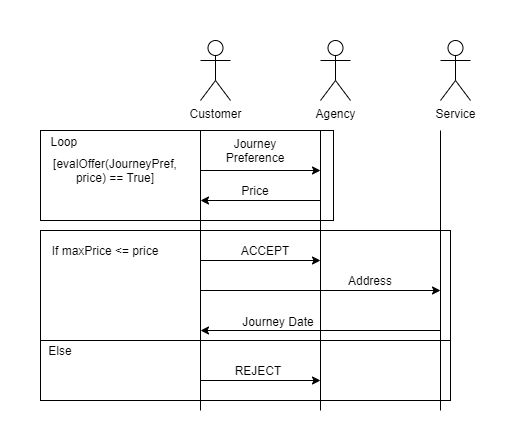
\includegraphics[scale=0.4]{Algorithm.png}
\caption{Plane Ticket Algorithm System Sequence Diagram}
\label{ssd}
\end{figure}
As we can see in figure \ref{ssd} the algorithm consists in an early stage of negotiation where a customer will send a journey preference(e.g. "Rome") to the agency and receive the price for a ticket to the given preference repeatedly until evalOffer evaluates to true.
At this point the customer will make a choice:
\begin{itemize}
\item If the received price is lower or equal to the max accepted price of the customer, he will accept the offer.
The agency will spawn a service which will receive the customer address and send the journey date.
\item If the received price is greater than the max accepted price of the customer, he will reject the offer and end the communication.
\end{itemize}
The pseudo code for this algorithm is as follow:
\begin{lstlisting}[caption={Customer Algorithm},captionpos=b]
class Customer {
	Address addr;
	double price, maxPrice;
	bool loop := true;
	String journeyPref;
	new Agency.sell {
		sendWhile (loop) {
			send( journeyPref );
			price := receive;
			loop := evalOffer(journeyPref,price);
			// implementation of evalOffer omitted
		};
		sendCase( evalPrice(price,maxPrice) ) {
			ACCEPT > send( addr ); Date date := receive;
			REJECT > null; /* customer rejects price
					,end of protocol */ 
		}
	} /* End method invocation */
}
\end{lstlisting}
\begin{lstlisting}[caption={Agency Algorithm},captionpos=b]
class Agency {
	String journeyPref;
	void acceptOrder sell {
		receiveWhile {
			journeyPref := receive;
			double price := getPrice( journeyPref );
			// implementation of getPrice omitted
			send( price );
		}
		receiveCase (x) { // buyer accepts price
			ACCEPT < new Service . orderDelivery { } ,
			REJECT < null;// receiveCase : buyer rejects 
        }
	} /* End method sell */
}
\end{lstlisting}
\begin{lstlisting}[caption={Service Algorithm},captionpos=b]
class Service {
	void receiveOrderSession orderDelivery() {
		Address custAddress := receive;
		Date date := new Date();
		send( date );
	}
}
\end{lstlisting}
\subsection{Programming Languages}
\subsubsection{Rust}\hfill\\\\
\subsubsection{Go}\hfill\\\\
Go is a programming language designed at Google that focuses in performance, usability and parallel programming.
It introduces a new primitive called Goroutines, a form of lightweight threads, meaning they share context with other goroutines in a program. They are also managed by the Go runtime, that will be responsible for the scheduling of each goroutine. This means that if one goroutine is blocked, Go's run-time will switch to another with work to do.
Goroutines multiplex coroutines, independently executing functions, onto a set of thread that by default match the number of logical processors of the environment. Of course this can be change with the {\bf GOMAXPROCS} function that sets the number of logical processes that the go program can access. Another great aspect of goroutines is that they achieve all this we a very modest amount of memory, allowing the execution of a great number of them.\\
Go treats channels are first class objects, in contrast with most of the other languages that offer them through external packages, or crates as we will see in Rust. This channels allow goroutines to communicate between themselves and it also allows to synchronize this same goroutines, because the channels block until the sender/receiver are ready to continue.\\	
Go was also built to be simple to understand, and because of that its syntax is very easy to learn. We can observe this in goroutines that can be started with a simple {\bf go func()} or the channels, constructed with {\bf make(chan type)}.
This language also encourages developers to write good code, emitting warnings to bad practices such as unused variables or unused imports, keeping the code clean.
\subsubsection{FreeST}\hfill\\\\

\textcolor{red}{FreeST is also a statically typed (certo?	), concurrent programming language. But it is not an imperative language, it is a functional language where processes communicate via message-passing through rendezvous channels. These channels are bidirectional and session types can be defined to specify how the channels will work.(É para os canais que se utilizam os Session types correto? Para definir protocolos)}
\section{Implementation Details}
\lipsum[1]
\subsection{Go}
\lipsum[1]
\subsection{Rust}
\lipsum[1]
\subsection{FreeST}
\lipsum[1]
\subsection{Discussion}
Here you should discuss the results on a high level. For instance, based on our results, the parallelization of the merge-sort is relevant as no other parallel work occurs at the same time, and the complexity $O(N log(N))$ can have a large impact when the number of individuals is high.
\section{Conclusions}
Here you should resume the major conclusions taken from discussion. Ideally, these should align with the objectives introduced in the introduction.


You should also list the future work, i. e., tasks and challenges that were outside your scope, but are relevant.
\section*{Acknowledgements}
First Author wrote the part of the program implemented the phasers. Second Author implemented the MergeSort in parallel. 

Both authors wrote this paper, with First Author focusing on the introduction, related work and conclusions while the Second Author focused on approach and evaluation.

Each author spent around 30 hours on this project.

\textcolor{red}{Jorge Martins implemented the algorithm in Rust and Go. Both authors implemented the algorithm in FreeST.
Both authors wrote this paper, ... 
Jorge Martins spent around X hours on this project. Diogo Lopes spent around Y hours on this project.}
\bibliographystyle{unsrt}
\bibliography{bibliography}
\end{document}